%--------------------------------------------------------------------------------------------------------------------  
%--------------------------------------------------------------------------------------------------------------------

  \subsection{Requerimientos}  

\subsubsection{Preguntas}
  
 \begin{enumerate} 
    \item \textbf{ Proceso de sinterizado }
	\begin{enumerate}
	  \item \textbf{ ¿Que magnitudes físicas se deben medir? }
		\subitem	\textit{ Las magnitudes que el sistema de debe medir son: corriente que circula en el momento de la descarga y 
					tensión sobre la muestra. Se evaluará la posibilidad de medir temperatura sobre la muestra de existir un
					sensor de temperatura con una respuesta temporal adecuada.
			}

	  \item \textbf{ ¿Cual es el mínima corriente requerida para el proceso? }
		\subitem	\textit{ La importancia radica en la corriente de pico al momento de la descarga.
				}

	  \item \textbf{ ¿Cual es el máxima corriente de pico esperada? }
		\subitem	\textit{ La magnitud del pico de corriente eléctrica en la descarga estará comprendido entre 1KA y 10KA.
				}

	  \item \textbf{ ¿Cual es el orden de magnitud de la impedancia eléctrica de la muestra de polvos? }
		\subitem	\textit{ La muestra estará constituida por un material metálico por lo que su impedancia estará en el orden los los m$\Omega$.
				}

	  \item \textbf{ ¿Se experimentará con distintos tipos de polvos? }
		\subitem	\textit{ No, solo se utilizaran polvos de materiales metálicos.
				}

          \item \textbf{ ¿Qué materiales en particular se van utilizar como muestra a sinterizar? }
		\subitem	\textit{ Se utilizaran materiales basados en hierro (Fe).
				}

          \item \textbf{ ¿Se proyecta que a futuro se utilice otros materiales?¿Cómo afectaría esto al proceso? }
		\subitem	\textit{ No, este tipo de tecnología solo se puede aplicar a materiales de tipo metálico.
				}

          \item \textbf{ ¿Existe algún proceso por el cual se puede determinar que la muestra está sinterizada correctamente?¿Se desea implementar? }
		\subitem	\textit{ El resultado del proceso se validará con una batería de pruebas y estudios externos al proceso
					  que se le realizaran a la muestra.
				}

	  \item \textbf{ ¿Existirá un único banco de capacitores (descargar múltiples secuenciales)? }
		\subitem	\textit{ El sistema debe poder ser escalable. Se debe especificar que cambios se deben hacer en caso de decir escalar
					la capacidad de corriente del sistema en los cables de conexión , sensores y  en los contactores del dispositivo.
				}

	  \item \textbf{ ¿Con qué periodicidad se estima realizar el proceso (horas, días, semanas)? }
		\subitem	\textit{ Se estima unos 60 usos por mes.
				}

	  \item \textbf{ ¿En cuanto a la compresión mecánica, qué prensa se utilizará? }
		\subitem	\textit{ Se utilizara un prensado manual o automático, pero en ambos casos el proceso de prensado será externo al dispositivo.
				}

	  \item \textbf{ ¿El valor de presión que se establece antes de empezar la descarga, debe reajustarse durante el proceso?¿Cual tiene que ser este valor constante? }
		\subitem	\textit{ No, la muestra del polvo a sinterizar se compactar antes de la descarga.
				}


	\end{enumerate}
	  
      \item \textbf{ Interfaz de usuario }
	\begin{enumerate}
	  \item \textbf{ ¿Cómo se desea visualizar los datos obtenidos del proceso? }
		\subitem	\textit{ Se desea tener una aplicación de PC dedicada al monitoreo, control y administración del sistema.
					 La aplicación debe poder funcionar en las plataformas Windows y Linux.
				}

	  \item \textbf{ ¿Es necesario un que el sistema tenga un display ?¿ Y teclado? }
		\subitem	\textit{ Si para la administración básica del dispositivo. La administración y gestion compleja del dispositivo se hará
					 a traves de la PC.
				}

	  \item \textbf{ ¿Se necesita accionar en forma manual algún parámetro del proceso, Cuál? }
		\subitem	\textit{ No, la totalidad del proceso de sinterizado y el monitoreo de las magnitudes deber ser automático.
				}

	  \item \textbf{ ¿En necesario visualizar los datos en forma remota (vía Web)? }
		\subitem	\textit{ No es necesario ya que no seria de utilidad.
				}

	  \item \textbf{ ¿Se cuenta con bocas de red cerca de la zona de emplazamiento del dispositivo?¿Se planea hacerlo? }
		\subitem	\textit{ No.
				} 

	  \item \textbf{ Los datos de la experimentación, ¿Deben quedar guardados en el dispositivo o un servidor local? }
		\subitem	\textit{ Si, los datos se almacenaran en el dispositivo hasta su descarga mediante el programa de PC.
				}

	  \item \textbf{ ¿Es necesario tener la posibilidad de guardar los datos en un pendrive? }
		\subitem	\textit{ Si es de utilidad.
				}

	  \item \textbf{ ¿Se desea genera alguna extensión de archivo en particular? }
		\subitem	\textit{ Es deseable el formato CSV.
				}

	  \item \textbf{ ¿Cómo desea configurar el sistema de control? }
		\subitem	\textit{ -------------
				}

	  \item \textbf{ ¿Que parámetros del proceso se deben visualizar y cuales almacenar (magnitudes física)? }
		\subitem	\textit{ Se mostraran el estado de los parámetros en el display pero los datos relevados de la experimentación se
					  obtendrán mediante el programa de PC.
				}

	  \item \textbf{ ¿Qué parámetros de control tiene el proceso (condiciones que se deben cumplir para iniciar el proceso. Ejemplo: nivel de carga)? }
		\subitem	\textit{ -------------
				}

	  \item \textbf{ ¿Qué parámetros de control deberían ser establecidos de forma remota y cuales de forma local? }
		\subitem	\textit{ La configuración del sistema será mediante el programa de PC.
				}

	  \item \textbf{ ¿Se necesita accionar en forma manual algún parámetro del proceso?¿Cuál? }
		\subitem	\textit{ No.
				}

	\end{enumerate}
      
      \item \textbf{ Seguridad }
	\begin{enumerate}
	  \item \textbf{ ¿Es necesario algún parámetro de seguridad en especial?¿Qué es lo más crítico del proceso? }
		\subitem	\textit{ Debe cumplir la normativa de seguridad impuesta en el laboratorio.
				}

	  \item \textbf{ ¿El operario estará en el mismo ambiente de la experimentación? }
		\subitem	\textit{ Si.
				}

	  \item \textbf{ ¿Debe haber elementos contra incendios? }
		\subitem	\textit{ No son necesarios.
				}

	  \item \textbf{ ¿Es necesario un nivel de autorización para operar el dispositivo (login)? }
		\subitem	\textit{ Si.
				}

	\end{enumerate}
      
    \end{enumerate}


  \newpage

%--------------------------------------------------------------------------------------------------------------------  
%--------------------------------------------------------------------------------------------------------------------

  \subsection{Construcción de la Casa de calidad (análisis de valor y competitividad)}  

  \newpage


%--------------------------------------------------------------------------------------------------------------------  
%--------------------------------------------------------------------------------------------------------------------

  \subsection{Especificaciones funcionales y de diseño}  
  
  \subsubsection{Aspectos eléctricos}
      \begin{itemize}
	\item Tensión alimentación: 220VAC/50Hz.
	\item Consumo máximo: 1A.$*^{1}$
	\item Pico de corriente de sinterizado máximo: 1KA. $*^{2}$
	\item Impedancia máxima de la muestra: 1$\Omega$. 
	\end{itemize}
     
    \begin{tabbing}
      \= ----- \= ----- \= --------------------- \= \kill
      \> $*^{1}$:\>	El consumo máximo estará fijado por la fuente que se utilice y esta por el transformador. \\
      \> $*^{2}$:\>	La corriente máxima de pico de sinterizado puede ser incrementada hasta 10 kA si se amplía\\
         	\>\>	el banco de capacitores, se remplaza los contactores y el cableado correspondiente.\\
     \end{tabbing}

    \subsubsection{Almacenamientos de datos}
      
      \begin{itemize}
	\item Memoria flash en soporte SD Card.
	\item Memoria flash en soporte pendrive USB 2.0.
      \end{itemize}

    \subsubsection{Comunicación}
      
      \begin{itemize}
	\item Comunicación USB 2.0 con la PC. $*^{3}$
      \end{itemize}
    
      \begin{tabbing}
	\= ----- \= ----- \= --------------------- \= \kill
	\>$*^{3}$: \>Se utiliza un bridge RS232-USB interno. \\
       \end{tabbing}
	
    \subsubsection{Periféricos del dispositivo}
      \begin{itemize}
	\item Display gráfico de 128x64 pixels.
	\item Teclado de 4 teclas.
	\item Sensor de corriente.
	\item Sensores de tensión $\times$ 3.
	\item Sensor de temperatura.
      \end{itemize}

    \subsubsection{Interfases del dispositivo}
      \begin{itemize}
	\item Entrada de 0-5V $\times$ 3.$*^{4}*^{5}$
	\item Entrada de 5-20mA $\times$ 1.$*^{4}$
	\item Puertos UART $\times$ 3.$*^{6}$
	\item Bus $ I^{2}C $.$*^{6}$
      \end{itemize}

      \begin{tabbing}
       \= ----- \= ----- \= --------------------- \= \kill
	\> $*^{4}$: \>Interfases configurables desde el programa de PC. \\
	\> $*^{5}$: \>Interfases usadas para los sensores de tensión y corriente \\
	\> $*^{6}$: \>Interfases reservadas para usos futuros. \\
      \end{tabbing}

    \subsubsection{Seguridad}
      \begin{itemize}
	\item Descarga segura del banco de capacitores.
	\item Sirena sonora.
	\item Luces de señalización $\times$ 3.
	\item Banco de capacitores ubicados dentro del gabinete del dispositivo .
	\item Revestimiento eléctricamente aislante del gabinete del dispositivo.
	\item Protección contra corto circuito.
	\item Botón de parada de emergencia.
      \end{itemize}

    \subsubsection{Aspectos mecánicos}
      \begin{itemize}
	\item No se brinda la función de prensado de la muestra. $*^{7}$
	\item Gabinete con 4 ruedas. 
	\item No se brinda el recipiente contenedor de la muestra de polvo.
      \end{itemize}

      \begin{tabbing}
       \= ----- \= ----- \= --------------------- \= \kill
	\> $*^{7}$: \>  La muestra debe estar prensada previamente al momento de realizar el \\
	    \>\>	proceso sinterizado.\\
      \end{tabbing}

    \subsubsection{Aspectos de operativos}
      \begin{itemize}
	\item Uso máximo mensual: 60 veces. $*^{8}$
      \end{itemize}
    
      \begin{tabbing}
	\= ----- \= ----- \= --------------------- \= \kill
	\> $*^{8}$: \>Se estima un promedio de 2 usos diarios. \\
      \end{tabbing}

\newpage

    \subsubsection{Diagrama en bloques del sistema }

    \begin{figure}[h!]
    \centering
    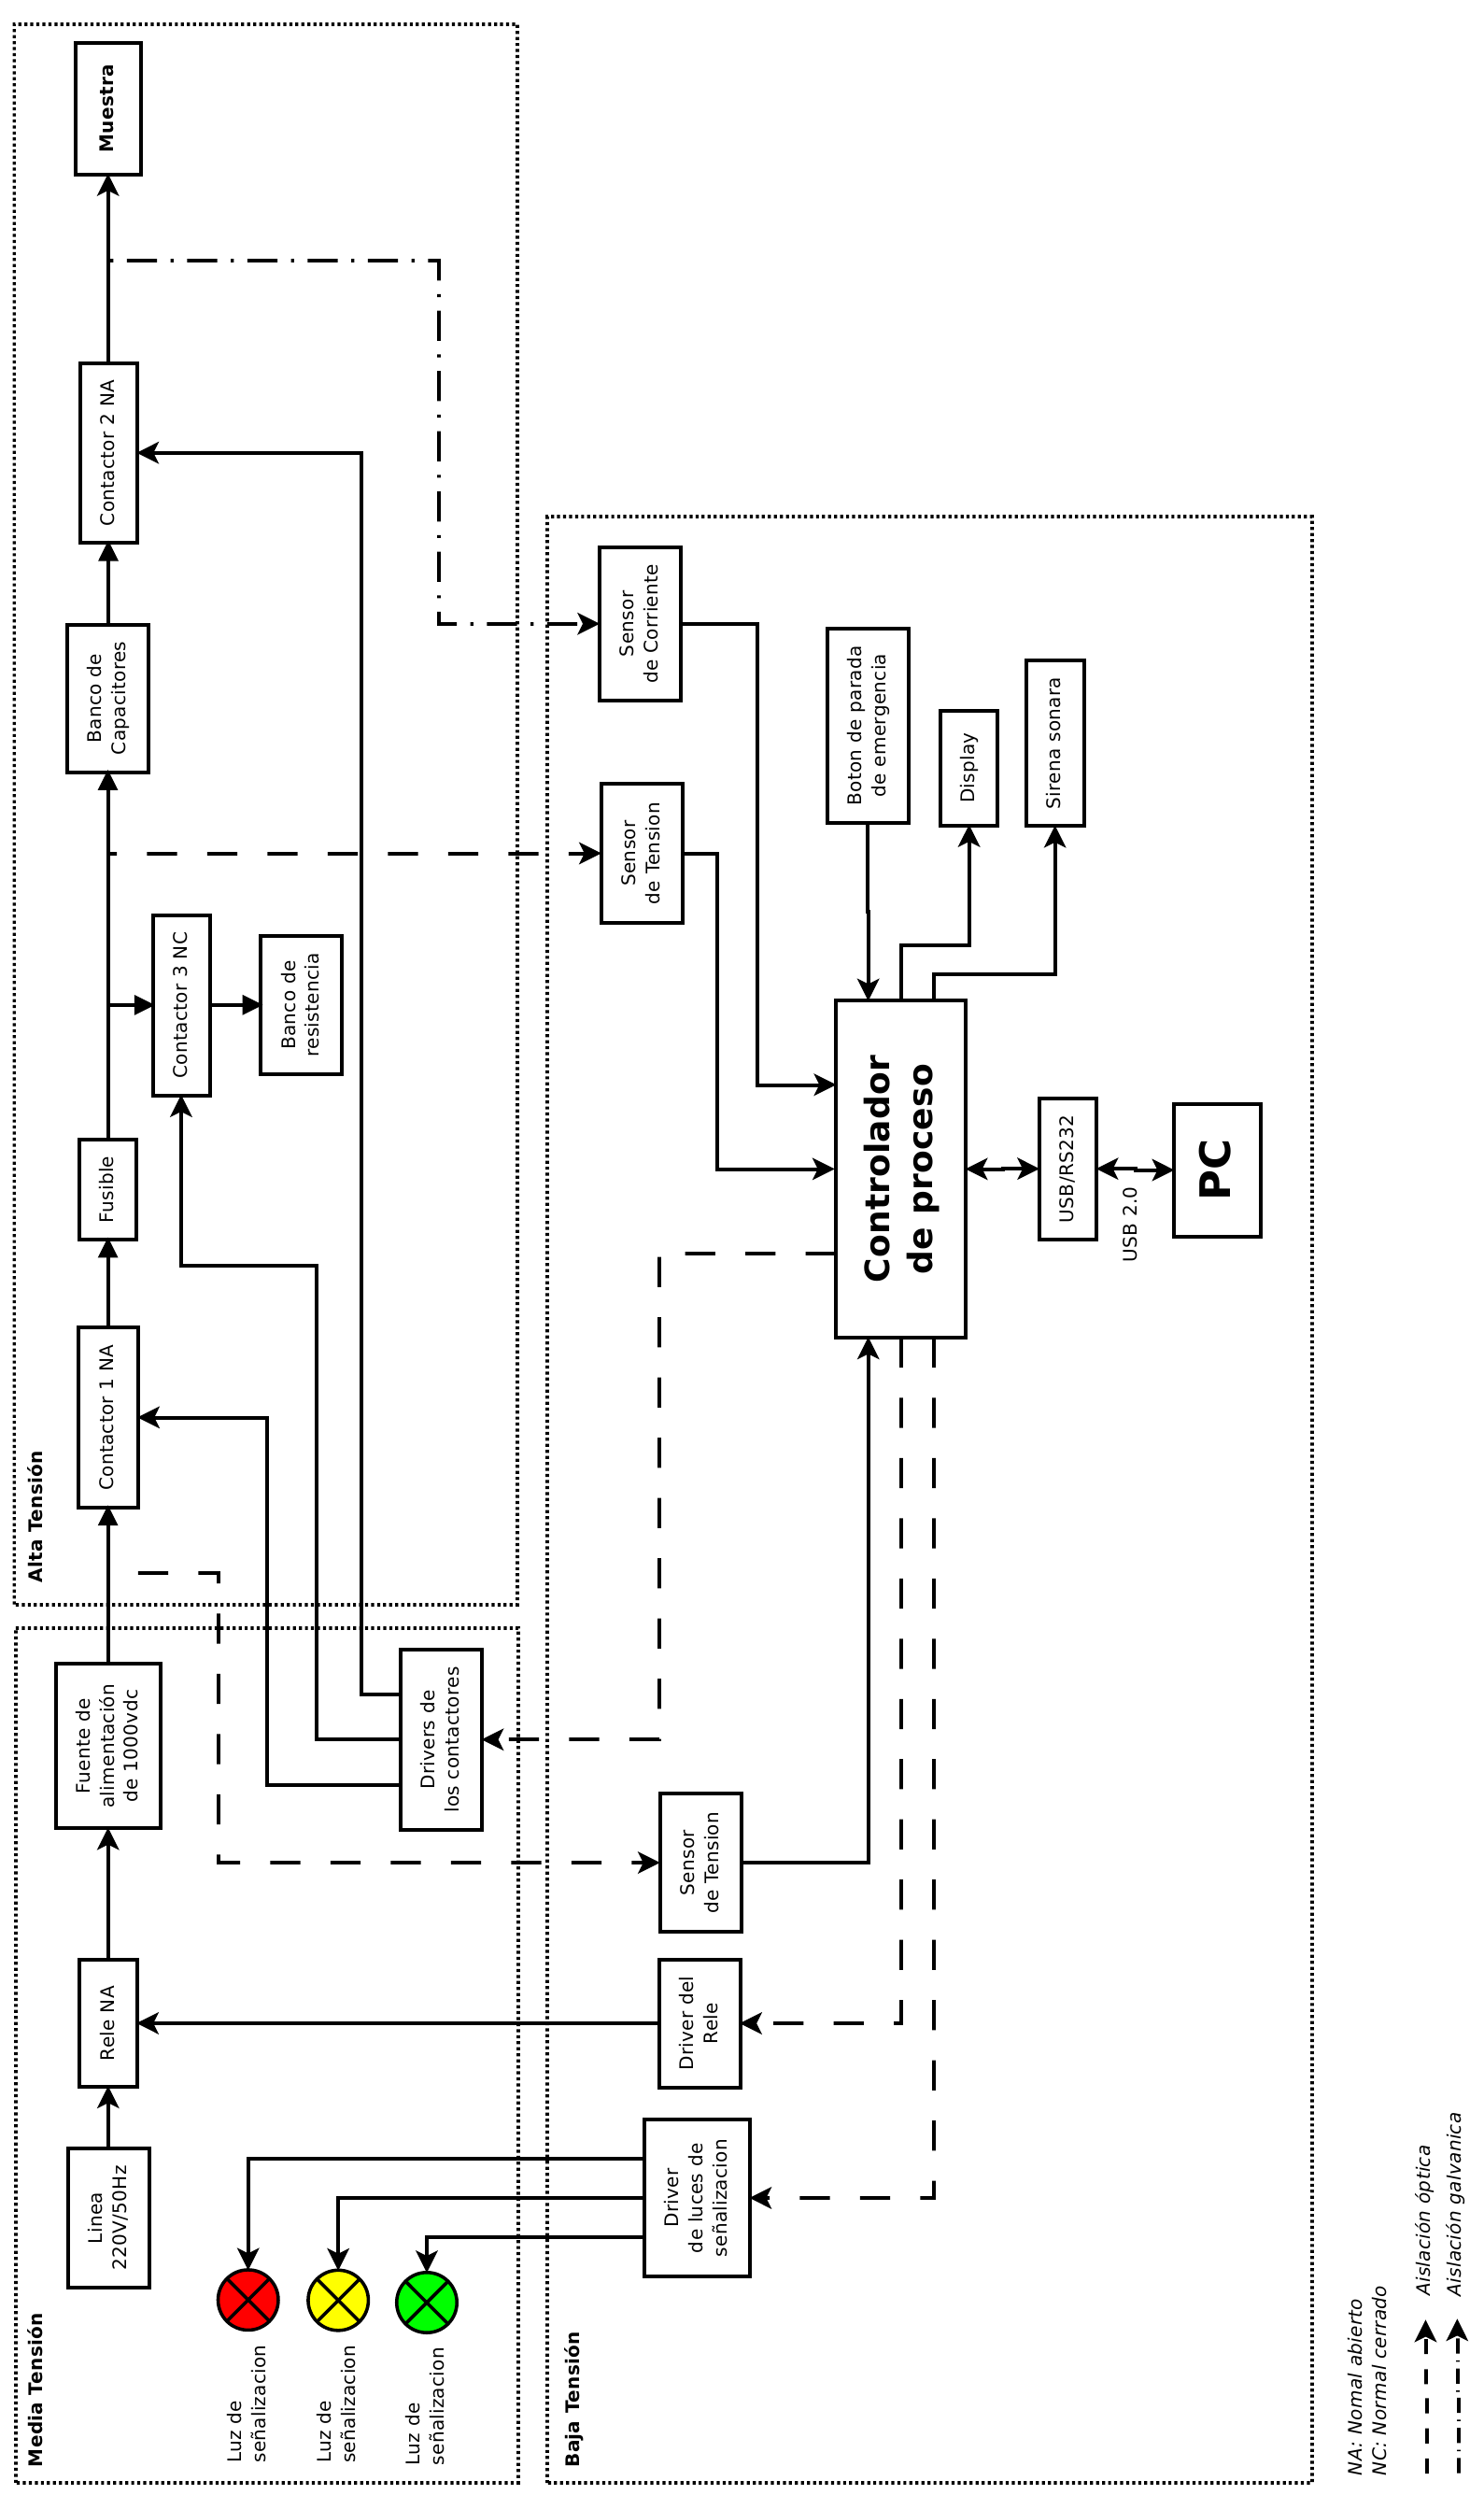
\includegraphics[width=370px]{../../Documentacion/Diagramas/diagramaBloquesDetalle.png}
    % diagramaBloquesEspecificaciones.png: 1170x708 pixel, 96dpi, 30.95x18.73 cm, bb=0 0 877 531
    \caption{Interconeccion entre los bloques del sistema}
    \end{figure}
  \newpage

%--------------------------------------------------------------------------------------------------------------------  
%--------------------------------------------------------------------------------------------------------------------

  \subsubsection{Especificación del software }  
 El control, administración, monitoreo y recolección de datos del dispositivo de control del proceso de sinterizado se harán a través de 
    un programa de PC con las siguiente características:
    
    \begin{itemize}
      \item Plataforma Windows XP/7 y GNU Linux.
      \item Formato de datos exportados CSV.
      \item Control de acceso.
      \item Base de datos.
    \end{itemize}
  
    \textbf{Pantallas}
      El programa contara con las siguientes pantallas: (FALTA AGREGAR LAS CAPTURAS DE LAS PANTALLAS)

    \begin{itemize}
      \item Login.      
      \item ABM usuarios.
      \item Monitoreo dispositivo.
      \item Parametrización del experimento.
      \item Control experimentación.
      \item Descarga de datos del experimento.
      \item Exportación de resultados de experimentación.
      \item Ploteo de resultados del experimento.
    \end{itemize}
  
  \newpage

%--------------------------------------------------------------------------------------------------------------------  
%--------------------------------------------------------------------------------------------------------------------  
%--------------------------------------------------------------------------------------------------------------------

 
%--------------------------------------------------------------------------------------------------------------------